\chapter{MATHEMATICAL MODEL}
In this project, a ship moving with a steady speed of $U$ in deep water with regular waves of wave amplitude $A$ and incident frequency $w_I$ traveling at an angle $\beta$ with the surge direction of the ship is considered. Potential flow methods are widely used to solve the seakeeping problem. Due to the improvement in the computation power, the three-dimensional boundary element method to compute the wave load can be used.

\section{Co-ordinate System}

In order to set up the mathematical model, two coordinate systems are defined; one of them is the Global coordinate system ( GCS ), whose origin is located at a calm water level. The other one is the Body seakeeping coordinate system ( BCS ), whose origin is located at the midship on the intersection of the water line and centerline of the ship. It is further assumed that the $x$-axis of the GCS points towards the east direction, whereas the $x$-axis of BCS points towards the sway direction of the ship. Coordinates of points represented in GCS are expressed as $\boldsymbol{x^e} = (x^e, y^e, z^e)$ wheres for the points in BCS it is expressed as $\boldsymbol{x^s} = (x^s, y^s, z^s)$. Global coordinate system, i.e., GCS, denotes the inertial frame of reference. Body geometry and body parameters, such as the location of the vertical center of gravity and radii of gyration, are defined with respect to BSC.

The translating frame of reference i.e. BCS allows the formulation of the vessel response in six degrees of freedom due to incident waves and steady current of speed $U$ in $-x$ direction which is equivalent to forward speed with respect to GCS. A linear boundary value problem can be introduced by assuming a small wave amplitude to determine the velocity potential.


\section{Velocity potential}
Assuming that the fluid flow is inviscid, incompressible, and irrotational the total velocity potential at any point inside the fluid domain is given as :
\begin{equation}
    \boldsymbol{\Phi} (\vec{x}, t) = [\, -Ux + \phi_P(\vec{x})\,] + [\, \phi_I(\vec{x}, \beta, \omega_I) + \phi_S(\vec{x}, \beta, \omega_I) + \sum_{j=1}^{6}n_j\phi_j(\vec{x}, U, \omega_e) \,]\, e^{i w_e t}
\end{equation}
In the above equation, $\omega_I$ denotes the encounter frequency, $\phi_P$ represents the perturbation potential due to steady translation, $\phi_I$ is the incident wave potential, $\phi_S$ is the scattering wave potential, $\phi_j$ and $n_j$ are the radiation wave potential due to unit motion and vessel motion amplitude respectively in $j^{th}$ direction.
Here, the perturbation potential $\phi_P$ has a relatively insignificant effect on total potential at low to moderate ship speed. Hence, it will be ignored to reduce the complexity of the problem. Hence, the final equation for velocity potential is given as :
\begin{equation}
    \label{eq:velocity_potential}
    \boldsymbol{\Phi} (\vec{x}, t) = -Ux + [\, \phi_I(\vec{x}, \beta, \omega_I) + \phi_S(\vec{x}, \beta, \omega_I) + \sum_{j=1}^{6}n_j\phi_j(\vec{x}, U, \omega_e) \,]\, e^{i w_e t}
\end{equation}
In the above equation, $\omega_e$ is the encounter frequency which is expressed in terms of incident or normal wave frequency $\omega_I$ , forward speed $U$, and incident angle $\beta$ as
\begin{equation}
    \label{eq:omega}
    \omega_e = \omega_I - \frac{\omega_I^2}{g}U\cos\beta
\end{equation}
\section{Governing equation}
The governing equations of the fluid flow are the continuity equation ( conservation of mass ) and the Navier-stokes equation ( conservation of momentum ). Under the assumption of inviscid and irrotational flow, the governing equations reduce to Laplace equations given as :
\begin{equation}
    \label{eq:laplace_eq}
    \nabla^2 (\phi_I, \phi_D, \phi_j) = 0
\end{equation}
where, $\phi_j \, (j = 1,2,\cdots, 6)$ denotes the radiation potential in all 6-modes of motion. This equation is valid over the entire fluid domain.

\section{Boundary Conditions}
\label{sec:Boundary condition}
In addition to the governing equation, the velocity potential satisfies the boundary conditions over the fluid boundaries. The total boundary surface $S$ comprises the free surface $S_F$, mean body surface $S_B$, bottom surface $S_Z$, and the radiation surface $S_\infty$ bounding the horizontal infinite fluid domain. The surfaces are shown in Fig. \ref{fig:boundary_surfaces} below.
\begin{figure}[H]
	\centering
	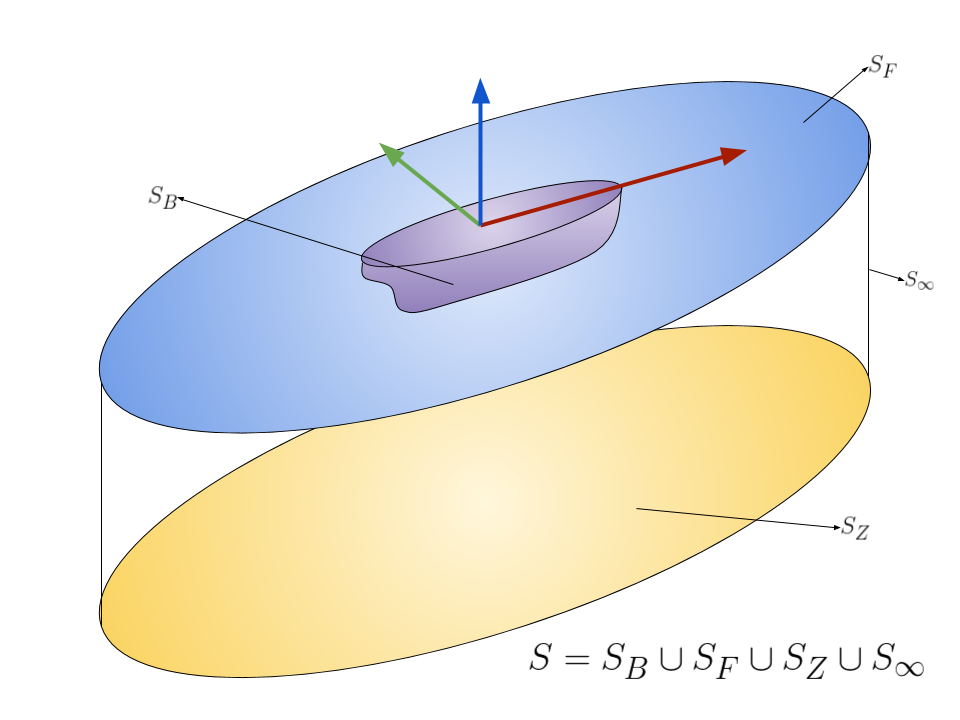
\includegraphics[width = 0.65\textwidth]{photos/boundary_surfaces.png}
	\caption{Fluid boundary surfaces}
	\label{fig:boundary_surfaces}
\end{figure}
The boundary conditions to be satisfied by the potential functions are shown below:

\begin{itemize}
    \item[1.] \underline{Kinematic free surface boundary condition} : 
    The velocity of the fluid in the direction normal to the free surface is equal to the velocity of the free surface. If the free surface is given by $z = \eta(t, x, y)$, then the boundary condition is given by
    \begin{equation}
        \label{eq:kin_free_surface_cond}
        \frac{\partial \eta}{\partial t} = \frac{\partial \phi}{\partial z} - \frac{\partial \phi}{\partial x} \frac{\partial \eta}{\partial x} - \frac{\partial \phi}{\partial y}\frac{\partial \eta}{\partial y} \quad \text{over} \; z
    \end{equation}
    
    \item[2.] \underline{Dynamic free surface boundary condition} : 
    The pressure obtained using Bernoulli's equations on the free surface is constant.
    \begin{equation}
        \label{eq:dyn_free_surface_cond}
        \left[\left(i\omega_e - u\frac{\partial}{\partial x}\right) + g\frac{\partial}{\partial z}\right](\phi_I, \phi_D, \phi_j) = 0 \quad \text{on} \; z = 0
    \end{equation}
    
    \item[3.] \underline{Radiation boundary condition} :
    The waves generated by the oscillating body propagate outward from the body to $\infty$ in the fluid domain, unbounded horizontally. This boundary condition is also referred to as the Sommerfeld radiation condition.
    \begin{equation}
        \label{eq:sommerfel_rad_cond}
        \lim_{kr\rightarrow \infty}\sqrt{kr}\left(\frac{\partial}{\partial r} -jk\right)(\phi_j - \phi_I) = 0 \quad \text{for}\; i = 1, 2, \cdots 6
    \end{equation}
    
    % \newpage
    \item[4.] \underline{Bottom Boundary condition} :
    The normal velocity of the fluid at the bottom boundary is equal to the normal velocity of the boundary. For an impenetrable seabed in deep water, the normal velocity is zero, and the boundary condition is given by 
    \begin{equation}
        \frac{\partial \phi}{\partial z} = 0 \quad \text{over the bottom}\; z = -\infty
    \end{equation}
    \item[5.] \underline{Body surface boundary condition}:
    The velocity of the fluid in the direction normal to the body boundary is equal to the normal velocity of the body boundary over the instantaneous underwater surface $S$.
    \begin{align}
        \label{eq:body_surface_boundary_cond}
        &\frac{\partial \phi_j}{\partial n} = i\omega_e n_j + Um_j \quad \text{on}\; S \\
        &\frac{\partial \phi_I}{\partial n} + \frac{\partial \phi_D}{\partial n} = 0 \quad \text{on}\; S
    \end{align}
    where $\vec{n} = (n_1, n_2, n_3)$ is the unit normal pointing outward from the hull surface and $(n_4, n_5, n_6)=\vec{r}\times \vec{n}$. Here, $r$ is the position vector of a point on the surface.
    The linear incident wave potential satisfying the above boundary conditions is given by:
    \begin{equation}
        \phi_I = \frac{igA}{\omega_I} e^{-ik_I(x\cos \beta + y\sin \beta)}e^{kz}
    \end{equation}
\end{itemize}

 Here, $\omega_I$ represents the incident wave frequency, not the encounter frequency.
This forward speed boundary value problem can be solved using potential theory using infinite depth free surface green function. 

